\doublespacing
\setlength{\parindent}{1cm}

To understand Convolutional Neural Networks, we have to understand the following foundational ideas:

\begin{itemize}
  \item Convolution
  \item Pooling
  \item Jargon: padding, stride, filter, etc
\end{itemize}

In computer vision, we have used diverse techniques in the past on images to do object detection and image classification. One major problem with computer vision problems is that the input data can get really big. Suppose an image is of the size 68 X 68 X 3. The input feature dimension then becomes 12,288. This will be even bigger if we have larger images (say, of size 720 X 720 X 3). Now, if we feed this big input to a neural network, the number of parameters will swell up to a very large number (depending on the number of hidden layers and hidden units). This will result in more computational and memory requirements – not something most of us can deal with. \par

We begin by looking at edge detection as a simple example. The early layers of a neural network detect edges from an image. Deeper layers might be able to detect the cause of the objects and even more deeper layers might detect the cause of complete objects (like a person’s face). \par

\textbf{Edge Detection Problem}

In this section, we will focus on how the edges can be detected from an image. Suppose we are given the figure below:

\begin{figure}
  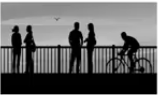
\includegraphics{edge-fig-1.png}
\end{figure}

As you can see, there are many vertical and horizontal edges in the image. Therefore, the first thing to be done is to detect these edges.

\begin{figure}
  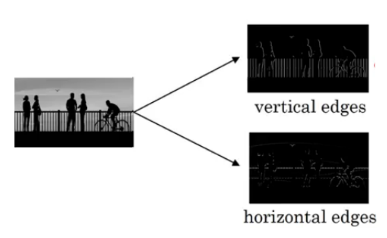
\includegraphics{edge-fig-2.png}
\end{figure}

How do we detect these edges? The first thing to do is assuming the image is BW, we represent it by a pixel map of gray scale values. Assume it is a 6 x 6 matrix.

\begin{figure}
  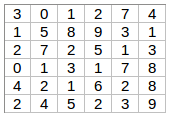
\includegraphics{matrix-fig-3.png}
\end{figure}

The values in these cells show pixel values in grayscale. Next, we convolve this 6 X 6 matrix with a 3 X 3 filter. They are also sometime referred to as feature detector or kernel.

\begin{figure}
  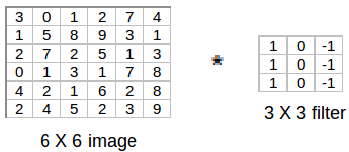
\includegraphics{mat-filter-fig-4.png}
\end{figure}

We take the feature filter and apply it over the original image. By placing it on the left upper corner, we get:

\begin{figure}
  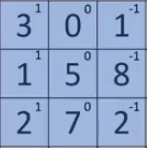
\includegraphics{mat-fig-5.png}
\end{figure}

So, we take the first 3 X 3 matrix from the 6 X 6 image and multiply it with the filter. Now, the first element of the output (which is a 4 X 4 matrix) will be the sum of the element-wise product of these values, i.e. 3*1 + 0 + 1*-1 + 1*1 + 5*0 + 8*-1 + 2*1 + 7*0 + 2*-1 = -5. To calculate the second element of the 4 X 4 output, we will shift our filter one step towards the right and again get the sum of the element-wise product:

\begin{figure}
  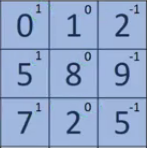
\includegraphics{mat-fig-6.png}
\end{figure}

Similarly, we will convolve over the entire image and get a 4 X 4 output:

\begin{figure}
  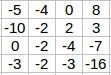
\includegraphics{mat-fig-7.png}
\end{figure}

The shifting of the filter is also called a stride. A stride of 1 shifts it one cell to the right, while a stride of 2 will shift it 2 cells to the right. So, convolving a 6 X 6 input with a 3 X 3 filter gave us an output of 4 X 4. This output is sometimes referred to as feature map. While the above explains what convolve operation does, we will take another example which can clarify how edges can be detected. If high pixel values represent bright areas and low values represent darker areas of an image, then look at this following example.

\begin{figure}
  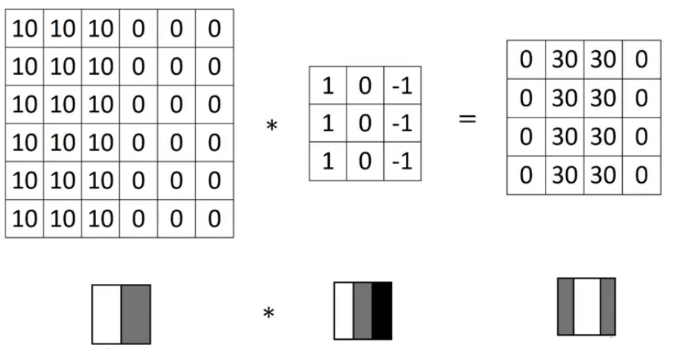
\includegraphics{conv-fig-8.png}
\end{figure}

Higher pixel values represent the brighter portion of the image and the lower pixel values represent the darker portions. Looking at the 4 x 4 output matrix, we can detect a vertical edge in an image.
\par
In mathematics, functional analysis,  convolution is a mathematical operation on two functions (f and g) to produce a third function that expresses how the shape of one is modified by the other. The convolution of f and g is written f∗g, using an asterisk or star. It is defined as the integral of the product of the two functions after one is reversed and shifted. As such, it is a specific kind of integral transform:
$$ [f*g](t) = \int_{0}^{t} f(\uptau) g(t - \uptau) \mathrm{d} \uptau $$


\begin{flushleft}
  \textbf{Kernel Types}
\end{flushleft}

A number of well-known filters or kernels have been used in prior work. Some common ones include Sharpen, Blue, Edge-Detect, or Edge-Enhance.

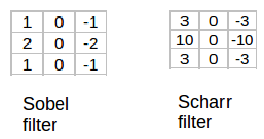
\includegraphics{filters-fig-9.png}

The Sobel filter puts a little bit more weight on the central pixels. Instead of using these filters, we can create our own as well and treat them as a parameter which the model will learn using backpropagation. In order to understand the next details of a CNN, let us take a look at the entire series of steps that happens on a single input image.
\par
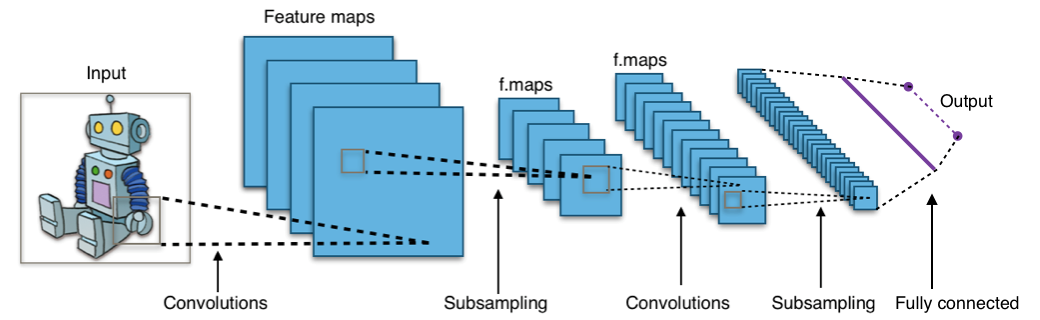
\includegraphics{cnn-fig-10.png}

It is important to note that a single image can generate many feature maps using different kernels. We do this so that different features are extracted out. This first step creates a convolutional layer consisting of many feature maps.
\par
\begin{flushleft}
  \textbf{Padding in Convolution}
\end{flushleft}

We have seen that convolving an input of 6 X 6 dimension with a 3 X 3 filter results in 4 X 4 feature map. We can generalize it and say that if the input is n X n and the filter size is f X f, then the output size will be (n-f+1) X (n-f+1):
\par
\begin{itemize}
  \item Input: n X n
  \item Filter size: f X f
  \item Output: (n-f+1) X (n-f+1)
\end{itemize}

There are two disadvantages to this approach:

\begin{enumerate}
  \item Every time a convolution is applied, the size of the image shrinks.
  \item Pixels present in the corner of the image are used only a few number of times during convolution as compared to the central pixels. Hence, not much focus is put on the corners since that can lead to a loss of information.
\end{enumerate}

In order to overcome these issues, we can pad the image with an additional border, i.e., we add one pixel all around the edges. This means that the input will be an 8 X 8 matrix (instead of a 6 X 6 matrix). Applying convolution of 3 X 3 on it will result in a 6 X 6 matrix which is the original shape of the image.
\par

This is where padding is very useful:

\begin{itemize}
  \item Input: n X n
  \item Padding: p
  \item Filter size: f X f
  \item Output: (n+2p-f+1) X (n+2p-f+1)
\end{itemize}

There are two common choices for padding.

\begin{enumerate}
  \item Valid: No padding at all. If we are using valid padding, the output will be (n-f+1) X (n-f+1)
  \item Same: Here, we apply padding so that the output size is the same as the input size, i.e., n+2p-f+1 = n ;therefore,  p = (f-1)/2
\end{enumerate}

We now know how to use padded convolution. This way we don’t lose a lot of information and the image does not shrink either. It is also important to note that the ReLU function (Rectifier Linear Function) is applied during the kernel application step since images are often very non-linear and we want to ensure that convolution does not create something too linear. Hence applying the ReLU rectifier function helps to solve this problem.

\begin{flushleft}
  \textbf{Pooling or Subsampling}
\end{flushleft}

Pooling layers are generally used to reduce the size of the inputs and hence speed up the computation. Consider a 4 X 4 matrix as shown below:

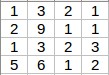
\includegraphics{mat-fig-11.png}

Applying max pooling on this matrix will result in a 2 X 2 output:

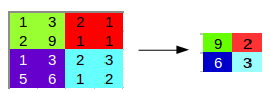
\includegraphics{max-pool-fig-12.png}

It is called max pooling as for every consecutive 2 X 2 block, we take the maximum number. Here, we have applied a filter of size 2 and a stride of 2. These are the hyperparameters for the pooling layer. Apart from max pooling, we can also apply average pooling where, instead of taking the max of the numbers, we take their average. In summary, the hyperparameters for a pooling layer are:

\begin{enumerate}
  \item Filter size
  \item Stride
  \item Max or average pooling
\end{enumerate}


If the input of the pooling layer is nh X nw X nc, then the output will be:
$$ \frac{(n_h – f)}{s + 1} \times \frac{(n_w – f)}{s + 1} \times n_c $$

In fact what max pooling does is that it takes features from convolutional layer and tries to pool all the relevant features and discard those that doesn’t help us in identification purposes.
